\section{Risultati e discussione: evoluzione della larghezza}
\label{sec:larghezza}
La larghezza di ogni tratto valido per ogni immagine disponibile, calcolata secondo l'equazione~\eqref{eq:larghezza-tratto}, viene riportata nel grafico in \cref{graph:larghezze-tutti-tratti}.
%
\begin{figure}
	\centering
	\tikzsetnextfilename{larghezze_tutti_tratti}
\begin{tikzpicture}
	\begin{axis}[
		width = .8\textwidth,
		height = \textwidth,
%		date coordinates in = y,
%		date ZERO = 2000-08-01,
%		yticklabel = {$\year-\month-\day$},
		yticklabel style = {
			rotate = 0,
			anchor = near yticklabel,
		},
		symbolic y coords = {2000-09-17, 2001-06-07, 2002-05-18, 2002-06-12, 2003-06-22, 2004-10-14, 2005-08-30, 2006-07-16, 2007-09-21, 2008-07-05, 2009-07-08, 2010-09-29, 2011-10-02, 2012-08-01, 2013-09-05, 2014-09-08, 2014-10-31, 2015-08-13, 2015-09-12, 2015-10-22, 2016-09-13, 2017-04-21, 2017-06-13, 2018-06-15, 2018-09-16},
		ytick distance = 1.5,
		xticklabel style = {font=\footnotesize},
		xtick = data,
		enlargelimits = 0,
		xlabel = {Tratto},
		colorbar right,
		]
		\addplot[
			matrix plot*,
			mesh/cols = 23,	% per fargli leggere colonne formate da 23 righe dal file di testo
			shader = flat corner,	% per interpolare i colori
		]
        	table [x = tratto, y = data, point meta = \thisrow{larghezza}] {graphics/data/Larghezze_tutti_tratti.txt};
	\end{axis}
\end{tikzpicture}

	\caption[larghezza di tutti i tratti per ogni immagine]{larghezza di tutti i tratti per ogni immagine; i quadrati bianchi indicano assenza di dati (a causa della presenza di nuvole o limitata estensione dell'immagine).}
	\label{graph:larghezze-tutti-tratti}
\end{figure}
%
\\
Ogni colonna del grafico corrisponde ad un'istantanea temporale: in quella specifica data, i tratti del Tagliamento avevano quella specifica larghezza.
Già così si vede quanto era stato descritto nell'introduzione:
i primi tratti sono quelli più stretti poiché confinati dalle montagne;
si osserva un progressivo allargamento all'incirca dal ponte autostradale di Braulins (a monte del tratto~6), interrotto dalla stretta di Pinzano (a valle del tratto~12);
infine, al successivo riallargamento dei tratti planiziali segue il cambio morfologico e il corrispondente restringimento (dal tratto~22).
Questo trend, costante nel tempo, viene mostrato nel grafico in \cref{graph:larghezza-2005-2018-09} per l'immagine \Se{} del 2018-09-16.
%
\begin{figure}
	\centering
	\tikzsetnextfilename{larghezza_2005_2018_09}
\begin{tikzpicture}
	\begin{axis}[
		width = \textwidth,
		height = 0.5\textwidth,
		xtick = data,
		enlarge x limits = 0.01,
		xlabel = {Tratto},
		ylabel = {Larghezza \si{[\m]}},
		grid = major,
		legend style = {
			at = {(0,1)},
			anchor = north west,		
		},
		]
		\addplot[
			purple,
			mark = star,
			]
        	table [x = tratto, y = larghezza_2005,] {graphics/data/larghezza_2005_2018_09.txt};
        \addlegendentry{2005-08-30};
        	
        	
		\addplot[
			blue,
			mark = star,
			]
        	table [x = tratto, y = larghezza_2018_09,] {graphics/data/larghezza_2005_2018_09.txt};
        \addlegendentry{2018-09-16};
        	
	\end{axis}
\end{tikzpicture}

	\caption[larghezza del tratto di studio nel 2005-08-30 e nel 2018-09-16]{larghezza del tratto di studio nell'immagine \AST{} 2005-08-30 e nell'immagine \Se{} 2018-09-16; si riconoscono i tratti più stretti a monte, presso la stretta di Pinzano (tra il tratto~12 e~13) e dove la morfologia diventa transizionale (tratti~22 e~23); questo trend è costante nel periodo di studio.}
	\label{graph:larghezza-2005-2018-09}
\end{figure}
%
\\
Considerando invece le righe, si può notare qualche specifico trend temporale (anche chiamato traiettoria evolutiva):
alcuni tratti intermedi, come l'8, il~9 o il~12, si sono allargati di diverse decine di metri negli ultimi anni;
i tratti~15, 16 e~17 hanno sperimentato la fusione di grandi isole nella piana alluvionale e quindi si sono ristretti di qualche centinaio di metri (\cref{fig:b-media-7-e-15}); sembra tuttavia che recentemente si siano riallargati.
Complessivamente non sembra che il fiume si stia particolarmente allargando o restringendo.
%
\begin{figure}
	\centering
	\begin{tikzpicture}
	\begin{axis}[
		width = 0.6\textwidth,
		height = 0.5\textwidth,
		date coordinates in = x,
		xticklabel = {\year},
		xticklabel style = {
			rotate = 80,
			anchor = near xticklabel
		},
		xtick distance = 730,
		enlarge x limits = 0.05,
		enlarge y limits = 0.01,
		%ymax = 3.7,
		%ymin = -0.1,
		%ytick distance = 0.5,
		ylabel = {Larghezza media dell'alveo \si{[\m]}},
		grid = major,
		]
		\addplot+
        	[blue]
        	table [x=data, y=tr_7] {graphics/data/Larghezze_medie_alveo.txt};
        \addlegendentry{Tratto 7}
        
		\addplot+
        	[orange]
        	table [x=data, y=tr_15] {graphics/data/Larghezze_medie_alveo.txt};
        \addlegendentry{Tratto 15}
	\end{axis}
\end{tikzpicture}

	\quad
	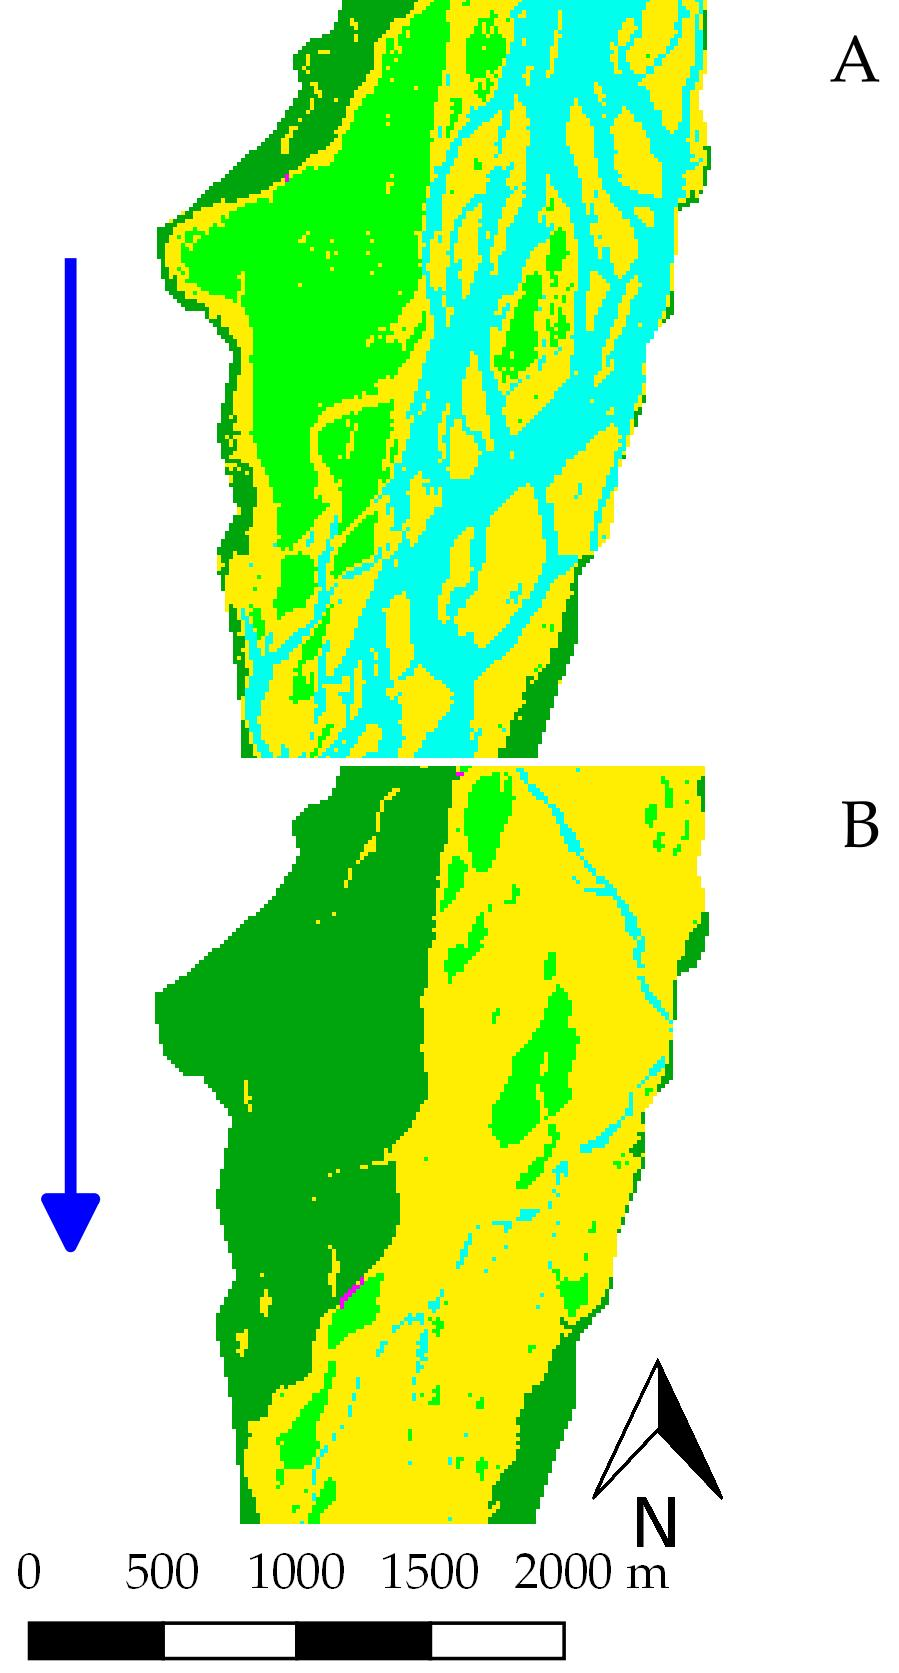
\includegraphics[width=0.3\textwidth]{files/fusione_isola_tr_15.jpeg}
	\caption[andamento temporale di $B$ per i tratti~7 e~15]{a sinistra si vede l'andamento nel tempo della larghezza media dell'alveo attivo $B$ dei tratti~7 e~15; la $B$ del tratto~7 oscilla solamente di qualche decina di metri, mentre il tratto~15 riduce improvvisamente la sua $B$ a causa della fusione di una grande isola nella \emph{floodplain}, fenomeno mostrato a destra (A: 2002-06-12, B: 2005-08-30).}
	\label{fig:b-media-7-e-15}
\end{figure}
%

È interessante confrontare alcuni risultati con quanto è stato svolto da altri autori: \squarecites{Zanoni:2008}{Surian:2015} riportano per i tratti dal~6 al~12 (dal ponte autostradale di Braulins alla stretta di Pinzano) la larghezza media ottenuta tramite la classificazione manuale di ortofoto aeree del secolo scorso e del decennio passato e tramite documenti catastali del 1800; è dunque possibile osservare traiettorie evolutive molto estese (\cref{graph:larghezze-vs-letteratura}).
%
\begin{figure}
	\centering
	\tikzsetnextfilename{larghezze_vs_letteratura}
\begin{tikzpicture}
	\begin{groupplot}[
		group style = {
			group size = 2 by 1,
			ylabels at = edge left,
			x descriptions at = edge bottom,
			horizontal sep = 0.5cm,
			vertical sep = 0.1cm,
		},
		width = 0.48\textwidth,
		height = 0.5\textwidth,
		date coordinates in = x,
		date ZERO = 1800-01-01,
		xticklabel = {$\year$},
		xticklabel style = {
			rotate = 80,
			anchor = near xticklabel
		},
		ylabel = {Larghezza \si{[\m]}},
		grid = major,
		]
		\nextgroupplot[
				legend columns = -1,
				legend to name = legend_larghezze,
				xtick distance = 18270,
			] % overview
			\addplot[green!70!black, mark = square*] % zanoni 2008
	        	table [x = data, y = larghezza] {graphics/data/largh_zanoni.txt};
	        	\addlegendentry{Zanoni et al. 2008}
			\addplot[orange, mark = triangle*] % surian 2015
	        	table [x = data, y = larghezza] {graphics/data/largh_surian.txt};
	        	\addlegendentry{Surian et al. 2015}
			\addplot[blue, mark = *] % mie
	        	table [x = data, y = larghezza] {graphics/data/largh_mie.txt};
	        	\addlegendentry{Presente tesi}
	        \draw [black, dashed, very thick] (1990-01-01,500) rectangle (2019-01-01,750);
	    %
		\nextgroupplot[
			xmin = 1990-01-01,
			ymin = 500,
			ymax = 750,
			yticklabel pos = right,
			xtick distance = 1827,
		] % zoom
			\addplot[green!70!black, mark = square*] % zanoni 2008
	        	table [x = data, y = larghezza] {graphics/data/largh_zanoni.txt};
			\addplot[orange, mark = triangle*] % surian 2015
	        	table [x = data, y = larghezza] {graphics/data/largh_surian.txt};
			\addplot[blue, mark = *] % mie
	        	table [x = data, y = larghezza] {graphics/data/largh_mie.txt};
	        \node [fill = white, draw = black, dashed, anchor = south east] 
        	at (axis description cs: 1,0) {Ingrandimento};
	\end{groupplot}
	%
	\draw [thick, blue, ->, shorten > = 2pt, shorten < = 2pt]
		(group c1r1.east) -- (group c2r1.west);
    %\node at ($(group c1r1) + (3.5cm,3.3cm)$) {\pgfplotslegendfromname{legend_larghezze}};
    \node at (group c1r1.north east) [anchor=south, xshift=.4cm] %.4cm è la metà della distanza orizzontale tra i plot
    	{\pgfplotslegendfromname{legend_larghezze}};
\end{tikzpicture}
	\caption[traiettoria evolutiva della larghezza media dell'area compresa tra il tratto~6 e il tratto~12]{traiettoria evolutiva della larghezza media dell'area compresa tra il tratto~6 e il tratto~12; sono presenti le traiettorie ottenute da \squarecite{Zanoni:2008} e da \squarecite{Surian:2015}.}
	\label{graph:larghezze-vs-letteratura}
\end{figure}
%
\\
Si vede chiaramente come i tratti si siano ristretti nel corso degli ultimi due secoli, forse a causa di lievi cambiamenti naturali nel regime idrologico, ma molto più probabilmente per le attività umane di prelievo di legname ed estrazione della ghiaia dall'alveo, avvenuti con particolare intensità nella seconda metà del 1900, così come degli interventi di ingegneria fluviale attuati dal 1950 (argini, soglie e opere di presa).
\\
In seguito, la concomitanza di piene importanti, della messa al bando dell'estrazione di ghiaia di fiume e della cessazione dell'utilizzo del legno presente in alveo per un cambiamento culturale ha indotto un graduale riallargamento di qualche centinaio di metri.
\\
I risultati in letteratura sono generalmente in accordo tra loro, così come non si discostano dai risultati della presente tesi.
Questi ultimi mostrano delle oscillazioni tra lievi allargamenti e restringimenti; sembra comunque che, anche negli ultimi \SI{20}{\anni} circa, questo tratto di fiume si stia ancora allargando, anche se ad un tasso sicuramente inferiore rispetto al decennio precedente.
Osservando proprio gli ultimi punti, si può quasi leggere un leggero restringimento; questo potrebbe essere reale, così come dovuto agli errori nella classificazione, data la modesta entità del cambiamento.
\\
Si nota una certa differenza tra le tre curve: alcuni punti degli altri lavori, punti che chiaramente provengono dalla classificazione delle medesime immagini, hanno valori di larghezza che differiscono di diverse decine di metri.
Questo può dipendere dal metodo di digitalizzazione dell'alveo e dalla definizione di isole, in particolare di quelle originatesi dal distacco di parte di piana alluvionale o di quelle in procinto di fondersi nella stessa.
Tuttavia, è la traiettoria evolutiva ciò che è importante evincere da questi risultati.
